%% USEFUL LINKS:
%% -------------
%%
%% - UiO LaTeX guides:          https://www.mn.uio.no/ifi/tjenester/it/hjelp/latex/
%% - Mathematics:               https://en.wikibooks.org/wiki/LaTeX/Mathematics
%% - Physics:                   https://ctan.uib.no/macros/latex/contrib/physics/physics.pdf
%% - Basics of Tikz:            https://en.wikibooks.org/wiki/LaTeX/PGF/Tikz
%% - All the colors!            https://en.wikibooks.org/wiki/LaTeX/Colors
%% - How to make tables:        https://en.wikibooks.org/wiki/LaTeX/Tables
%% - Code listing styles:       https://en.wikibooks.org/wiki/LaTeX/Source_Code_Listings
%% - \includegraphics           https://en.wikibooks.org/wiki/LaTeX/Importing_Graphics
%% - Learn more about figures:  https://en.wikibooks.org/wiki/LaTeX/Floats,_Figures_and_Captions
%% - Automagic bibliography:    https://en.wikibooks.org/wiki/LaTeX/Bibliography_Management  (this one is kinda difficult the first time)
%%
%%                              (This document is of class "revtex4-1", the REVTeX Guide explains how the class works)
%%   REVTeX Guide:              http://www.physics.csbsju.edu/370/papers/Journal_Style_Manuals/auguide4-1.pdf
%%
%% COMPILING THE .pdf FILE IN THE LINUX IN THE TERMINAL
%% ----------------------------------------------------
%%
%% [terminal]$ pdflatex report_example.tex
%%
%% Run the command twice, always.
%%
%% When using references, footnotes, etc. you should run the following chain of commands:
%%
%% [terminal]$ pdflatex report_example.tex
%% [terminal]$ bibtex report_example
%% [terminal]$ pdflatex report_example.tex
%% [terminal]$ pdflatex report_example.tex
%%
%% This series of commands can of course be gathered into a single-line command:
%% [terminal]$ pdflatex report_example.tex && bibtex report_example.aux && pdflatex report_example.tex && pdflatex report_example.tex
%%
%% ----------------------------------------------------


\documentclass[english,notitlepage,reprint,nofootinbib]{revtex4-2}  % defines the basic parameters of the document
% For preview: skriv i terminal: latexmk -pdf -pvc filnavn
% If you want a single-column, remove "reprint"

% Allows special characters (including æøå)
\usepackage[utf8]{inputenc}
% \usepackage[english]{babel}

%% Note that you may need to download some of these packages manually, it depends on your setup.
%% I recommend downloading TeXMaker, because it includes a large library of the most common packages.

\usepackage{physics,amssymb}  % mathematical symbols (physics imports amsmath)
\usepackage{amsmath}
\usepackage{graphicx}         % include graphics such as plots
\usepackage{xcolor}           % set colors
\usepackage{hyperref}         % automagic cross-referencing
\usepackage{listings}         % display code
\usepackage{subfigure}        % imports a lot of cool and useful figure commands
% \usepackage{float}
%\usepackage[section]{placeins}
\usepackage{algorithm}
\usepackage[noend]{algpseudocode}
\usepackage{subfigure}
\usepackage{tikz}
\usetikzlibrary{quantikz}
% defines the color of hyperref objects
% Blending two colors:  blue!80!black  =  80% blue and 20% black
\hypersetup{ % this is just my personal choice, feel free to change things
	colorlinks,
	linkcolor={red!50!black},
	citecolor={blue!50!black},
	urlcolor={blue!80!black}}


% ===========================================

%\addbibresource{refs.bib} % Entries are in the "refs.bib" file

\begin{document}
	
	\title{\Huge{Solving the Schrödinger Equation Using the 2D Crank-Nicolson Method}}  % self-explanatory
	\author{Eloi Martaillé Richard,
	\
	Christophe Kristian Blomsen,
	\
	Ola Mårem
	\&
	Jørgen Armann Glenndal
    }
	\date{\today}                             % self-explanatory
	\noaffiliation                            % ignore this, but keep it.
	
	%This is how we create an abstract section.
	\begin{abstract}
This paper solves the 2D time-dependent Schrödinger equation numerically for a single particle
	interacting through the different slits. To solve this PDE, we will apply the
	Crank-Nicolson method. For convergence check, we verified that the probability of finding our particle inside the box remains 1 at all times. The total probability was conserved within an
	error margin of  $10^{-14}$. We studied the particle's distribution probability at a certain time and explored the detection probability through our three kinds of slit setup.
	The code can be found in a GitHub repo:		\href{https://github.com/christopheblomsen/fys4150_pro5}{https://github.com/christopheblomsen/fys4150\_pro5}

\end{abstract}
	\maketitle	
	
	
	% ===========================================
	\section{Introduction} \label{sec:introduction}
	% ===========================================

	Light has always been an intriguing phenomenon in physics. It began in ancient Greece when Democritus argued that all things in the universe are composed of indivisible
	sub-components, i.e., particles. At the beginning of the eleventh century Ibn al-Haytham
	wrote a physics book describing light no longer as a particle but as a wave, using a
	pinhole lens to reflect, and refract rays of light. This started a heated debate about the
	wave-particle duality of light. All physicists joined one of the two sides and tried to
	prove that light was either a wave or a particle. \\

	In 1801, Thomas Young developed the double-slit experiment from the Huygens-Fresnel principle
	resulting in the discovery of wave interference of light\cite{ThomasYoung}.


	This experiment did not solve the debate, but the wave property of light began to dominate
	scientific thinking. We will need the introduction of Quantum Mechanics to show that
	light can behave as a particle and as a wave, with the Schrödinger'equation being derived
	from the wave equation. \\

	In this report, we use the 2D time-dependent Schrodinger's equation to simulate a particle's
	motion in different slit methods, namely no slit, one, two or three slits. Since the equation is a PDE, similar to the heat equation, we will apply the Crank-Nicolson method.
Originally this finite difference method was used to solve the heat equation\cite{Crank1947APM}. \\

	In section \ref{sec:theory} we will overview the theoretical aspect of our problem by introducing
	the Schrödinger equation with some light quantum mechanical motion. Then in section \ref{sec:methods}
	we will introduce the numerical solution applied with the Crank-Nicolson method and the simulation. After that, we will briefly introduce all results obtained from the simulation in the section
	\ref{sec:results}. Finally, we will discuss those results in section \ref{sec:discussion}, and
	in section  \ref{sec:conclusion}, we provide a summary.

	% ===========================================
	\section{Theory} \label{sec:theory}
	% ===========================================
	The time-dependent Schrödinger equation is defined as

	\begin{equation}
	i \hbar \frac{d}{d t}|\Psi\rangle=\hat{H}|\Psi\rangle \label{eq:schro_eq}
	\end{equation}

	where $\hat{H}$ is the Hamiltonian operator representing the total energy of the system
	and $|\Psi\rangle$ is the vector state in the Hilbert space. $|\Psi\rangle$ is a vector
	containing all possible information on the system at a specific time $t$. However, the actual physical meaning of $|\Psi\rangle$ remains an open question as it is impossible to
	physically observe $|\Psi\rangle$ \cite{griffiths:quantumn}. To obtain the information
	from $|\Psi\rangle$, we have to apply a certain operator on it, giving us a probability
	through the Born rule.\\


	In this paper, we will consider the case of a single, non-relativistic particle in two dimensions.
	We will also work in the position space to express our vector
	in terms of the orthonormal basis of the position space $|x_i\rangle$. This allows us
	, from the Born rule to calculate the probability of finding our particle between
	$x_i$ with the discretization of  $|\Psi\rangle$  at time $t_n$

	\begin{equation}
		P(x_i;t_n) = \langle x_i |\Psi\rangle = |\Psi^n_i|^2 =  \Psi^{n\dagger}_i\Psi^n_i
	\end{equation}

	with $\Psi^\dagger$ being the complex-conjugate and assuming normalization of $
	|\Psi\rangle$. \\

	By expressing our 2D Hamiltonian operator, we can then rewrite our eq. \ref{eq:schro_eq}


	\colorbox{red}{look ugly}

	\begin{align*}
		& \quad i \hbar \frac{\partial}{\partial t} \Psi(x, y, t)= \\
		& \left[-\frac{\hbar^{2}}{2 m}\left(\frac{\partial^{2}}{\partial x^{2}}+\frac{\partial^{2}}{\partial y^{2}}\right)+V(x, y, t)\right] \Psi(x, y, t) \tag{2} \label{eq:explicit_scho}
	\end{align*}


	To simplify our simulation, we will scale away all dimensions in \eqref{eq:explicit_scho}.
	
	% ===========================================
	\section{Methods}\label{sec:methods}
	% ===========================================
	\subsection{The Bare Schrödinger Equation}
	The bare Schrödinger equation is dimentionless and can be written as 

	\begin{equation}\label{eq:bare Schrodinger}
		\begin{split}
		i \frac{\partial u}{\partial t} &= -\frac{\partial^2 u}{\partial x^2} - \frac{\partial^2 u}{\partial y^2} + v(x,y) u\\
		\Rightarrow \ \ \frac{\partial u}{\partial t} &= i\left(\frac{\partial^2 u}{\partial x^2} + \frac{\partial^2 u}{\partial y^2}\right) - iv(x,y) u.
		\end{split}
	\end{equation} 
	
	\noindent
	In order to solve equation \ref{eq:bare Schrodinger} numerically, we must discetize all the terms and approximate
	the derivatives. The discretization is done by introducing a grid of points in the
	$xy$ plane containing all the values of $x$ and $y$ we will use. The time is discretized by using points, with equal spacing, along the time axis.\\ \\
	The first order time derivative on the left hand side of equation \ref{eq:bare Schrodinger} is approximated using the forward Euler method given by
	\begin{equation}
		\frac{\partial u^{n}}{\partial t} \approx \frac{u^{n+1}-u^n}{\Delta t},
	\end{equation}

	\noindent
	where $u^n$, in our case, is the dimensionless wave-function in two dimensions.
	The superscript denotes the time step of $u$ and $\Delta t$ is the length of the time
	step, i.e. the spacing between points on the time axis.	For the second order spatial derivatives
	on the right hand side of equation \ref{eq:bare Schrodinger}
	we use Taylor approximations of second order. In the $x$ direction,
	the double spatial derivative is then given by
	
	\begin{equation}\label{ex:double x}
		\frac{\partial^2 u_{i,j}}{\partial x^2} \approx \frac{u_{i+1,j}-2u_{i,j}+u_{i-1,j}}{h^2},
	\end{equation}
	where the subscript denotes the $x$ and $y$ spatial step and $h$ is the spatial step size.
	The equation for the $y$ direction is a matter of flipping the variables from
	$x \rightarrow y$ and $i \rightarrow j$.
	in equation \ref{ex:double x}.
	\subsection{The Crank-Nicolson Approach}
	
	\noindent
	The approximations for the derivatives are used in
	the Crank-Nicolson approach, which is given by
	
	\begin{equation}
		\frac{u^{n+1}-u^{n}}{\Delta t} = \frac{1}{2}    \left(     F^{n+1} + F^n     \right),
	\end{equation}

	\noindent
	where the $F^{n+1}$ and $F^n$ terms are the right hand side of equation \ref{eq:bare Schrodinger}
	evaluated at the specified time steps. The superscript denotes the time step of the given variable, and $\Delta t$ is the length of the time step,
	i.e. the spacing between points on the time axis.\\ \\

	\noindent
	Rewriting equation \ref{eq:bare Schrodinger}
	according to the Crank-Nicolson approach we get 
	\begin{equation}\label{eq:algo}
		\begin{aligned}
		\frac{u^{n+1}_{i,j}-u^{n}_{i,j}}{\Delta t} &=  \frac{1}{2}\Big(\left(i\left(\frac{\partial^2 u_{i,j}}{\partial x^2} + \frac{\partial^2 u_{i,j}}{\partial y^2}\right) -i v_{i,j} u_{i,j}\right)^{n+1} \\
	    &+   \left(i(\frac{\partial^2 u_{i,j}}{\partial x^2} + \frac{\partial^2 u_{i,j}}{\partial y^2}) -i v_{i,j} u_{i,j}\right)^{n} \Big)\\
	    &\ \\
		&=  \frac{1}{2}\Big(    \frac{i}{h^2}\big(  u^{n+1}_{i+1,j}-2u^{n+1}_{i,j}+u^{n+1}_{i-1,j}   +u^{n+1}_{i,j+1}\\
		&-2u^{n+1}_{i,j}+u^{n+1}_{i,j-1}\big)-iv_{i,j}u^{n+1}_{i,j}\\
		&+ \frac{i}{h^2}\big(  u^{n}_{i+1,j}-2u^{n}_{i,j}+u^{n}_{i-1,j}   +u^{n}_{i,j+1}\\
		&-2u^{n}_{i,j}+u^{n}_{i,j-1}\big)-iv_{i,j}u^{n}_{i,j}      \Big)\\ 
		&\ \\
		&\Rightarrow \\ 
		&\ \\
		&u^{n+1}_{i,j} -r\Big(  u^{n+1}_{i+1,j}-2u^{n+1}_{i,j}+u^{n+1}_{i-1,j} \\
		&+u^{n+1}_{i,j+1}-2u^{n+1}_{i,j}+u^{n+1}_{i,j-1}\Big) +\frac{i\Delta t}{2}v_{i,j}u^{n+1}_{i,j}\\
		&\ \\
		&= u^n_{i,j}+ r\Big(  u^{n}_{i+1,j}-2u^{n}_{i,j}+u^{n}_{i-1,j}\\
		&+u^{n}_{i,j+1}-2u^{n}_{i,j}+u^{n}_{i,j-1}\Big)-\frac{i\Delta t}{2}v_{i,j}u^{n}_{i,j},
		\end{aligned}
	\end{equation}
	\noindent
	where we have used that $r = \frac{i\Delta t}{2h^2}$. The terms at time
	step $n+1$ are on the left hand side and terms at time step $n$ are on the right
	hand side.\\
	

	\subsection{The Simulated System}

	\noindent
	By using the Dirichlet boundary conditions in the $xy$ plane, i.e.
	\begin{itemize}
		\item $u(x=0, y, t) = 0$
		\item $u(x=1, y, t) = 0$
		\item $u(x, y=0, t) = 0$ 
		\item $u(x, y=1, t) = 0$,
	\end{itemize}
	we can write the result of equation \ref{eq:algo} as a matrix
	equation on the form 
	\begin{equation}
	Au^{n+1} = Bu^n,	
	\end{equation} 
	which can easily be solved when the initial condition of $u$ is known.\\ \\
	\noindent
	For the initial condition of the dimensionless wave-function in two dimensions,
	i.e. $u^{0}$, we use an un-normalized Gaussian wave packet given by

	\begin{equation}\label{eq:wave packet}
		u(x,y,t=0) = e^{-\frac{(x-x_c)^2}{2 \sigma_x^2} - \frac{(y-y_c)^2}{2 \sigma_y^2} + i p_x (x-x_c) + i p_y (y-y_c)}.
	\end{equation}
	
	\noindent
	In equation \ref{eq:wave packet}, $x_c$ and $y_c$ are the central
	coordinates of the wave packet, $\sigma_x$ and $\sigma_y$ are the standard
	deviations in the $x$ and $y$ directions respectively and $p_x$ and $p_y$
	are the momenta of the wave packet. Since we use dimentionless units, we let 
	$x \in [0,1]$, $y \in [0,1]$ and $t \in [0,T]$.\\ \\
	
	\noindent
	The potet


	
	
	% ===========================================
	\section{Results}\label{sec:results}
	% ===========================================
	We now present the results for the open box, and the two-slit system, using the initial conditions in table \ref{tab:1}.
	\begin{table}[h!]
	\centering
	\caption{system parameters used for calculating the probability distribution for the no-slit and double slit.}
	\label{tab:1}
	\begin{tabular}{c | c | c} %Frode uses vertical lines, therefore, we can do it
	 Variable& No slit & Double slit\\
	\hline
	$h$                & $5\cross10^{-3}$                &\quad $5\cross10^{-3}$   \\
	$\Delta t$       & $2.5\cross10^{-5}$            &\quad $2.5\cross10^{-5}$  \\
	$T$                & $8\cross10^{-3}$               &\quad $8\cross10^{-3}$     \\
	$x_c$             & $2.5\cross10^{-1}$            &\quad $2.5\cross10^{-1}$  \\
	$\sigma_x$    & $5\cross10^{-2}$               &\quad $5\cross10^{-2}$     \\
	$p_x$             & $2\cross10^{2}$                &\quad $2\cross10^{2}$      \\
	$y_c$             & $5\cross10^{-1}$               &\quad $5\cross10^{-1}$     \\
	$\sigma_y$    & $5\cross10^{-2}$               &\quad $1\cross10^{-1}$     \\
	$p_y$             & $0$                                    &\quad $0$                         \\
	$v_0$             & $0$                                    &\quad $1\cross10^{10}$    \\
	Wall thickness      & $2\cross10^{-2}$               & $2\cross10^{-2}$        \\
	Slit aperture          & $0$                                     & $5\cross10{-2}$        \\
	Wall between slits & $5\cross10^{-2}$          & $5\cross10^{-2}$            \\
	\hline
	\end{tabular}
	\end{table}
	The resulting absolute error of these systems can, as functions of time, be seen in figure \ref{fig:prob7_error}.
	
	\begin{figure}[H]
		\centering
		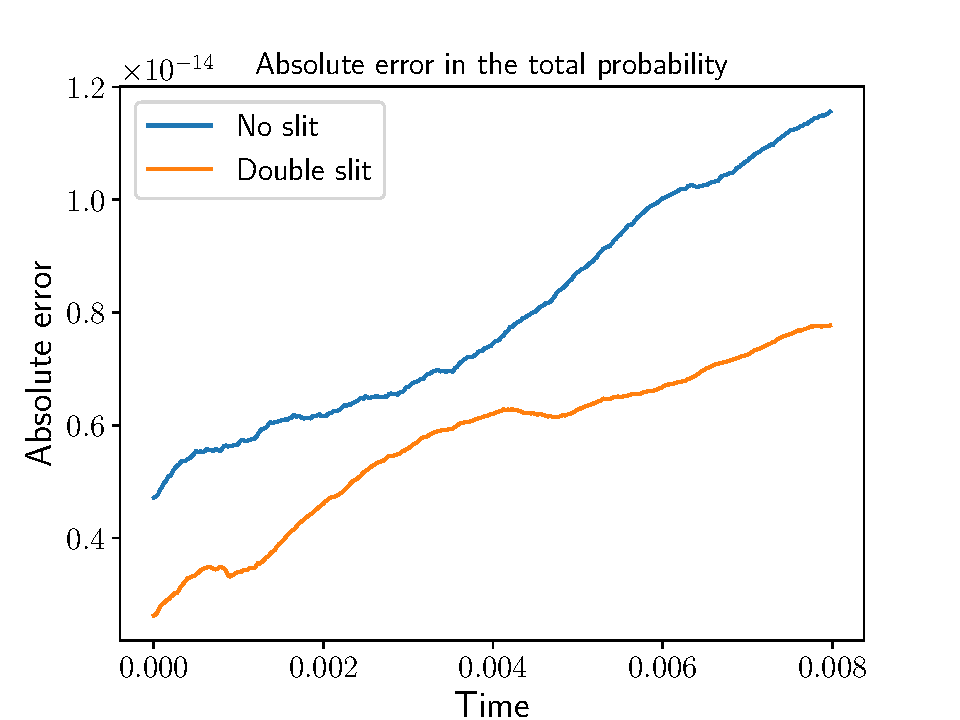
\includegraphics[scale=0.55]{figures/problem7_error.pdf}
		\caption{Absolute error versus time, using the system parameters in table \ref{tab:1}}
		\label{fig:prob7_error}
	\end{figure}
	We then find how the wave packet probability propagates through the two-slit system. First at time $t=0$.

	\begin{figure}[H]
		\centering
		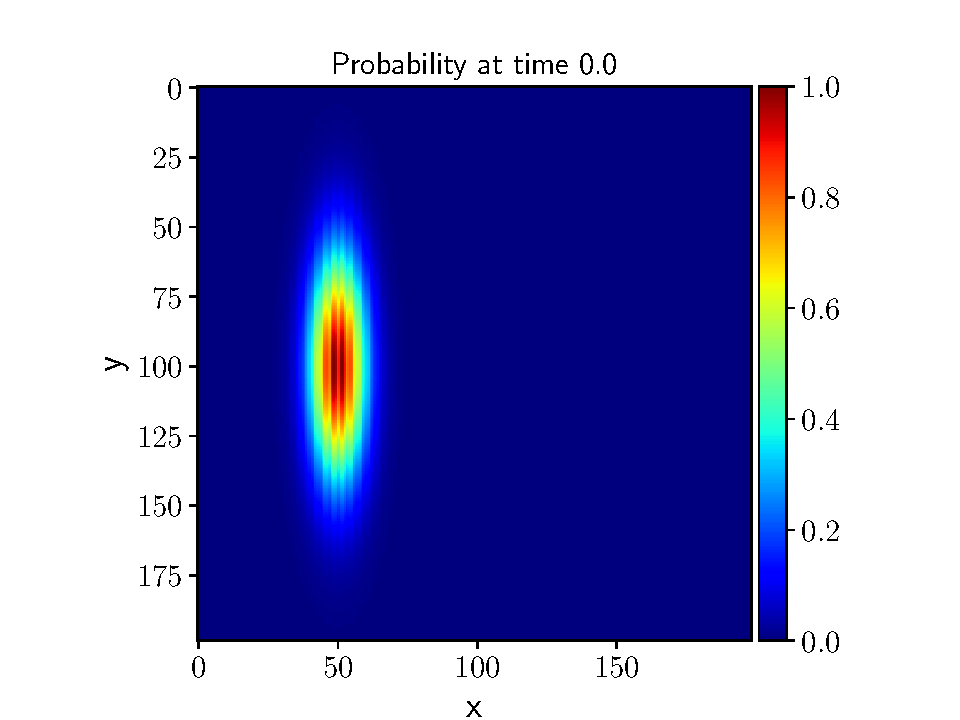
\includegraphics[trim={1cm 0cm 1cm 0cm},clip,width=0.49\textwidth]{figures/prob_plot_0.0.pdf}
		\caption{}
		\label{fig:prob_P0}
	\end{figure}
	Here, $x$ and $y$ are defined as dimensionless position, $x, y\in[0, 1]$ in units pixels. We have then the system at time $t = 10^{-3}$ in figure \ref{fig:prob8_P1}. The particles position is observed to have a probability on both sides of the slits, as well as the origin of a interference pattern.

	\begin{figure}[H]
		\centering
		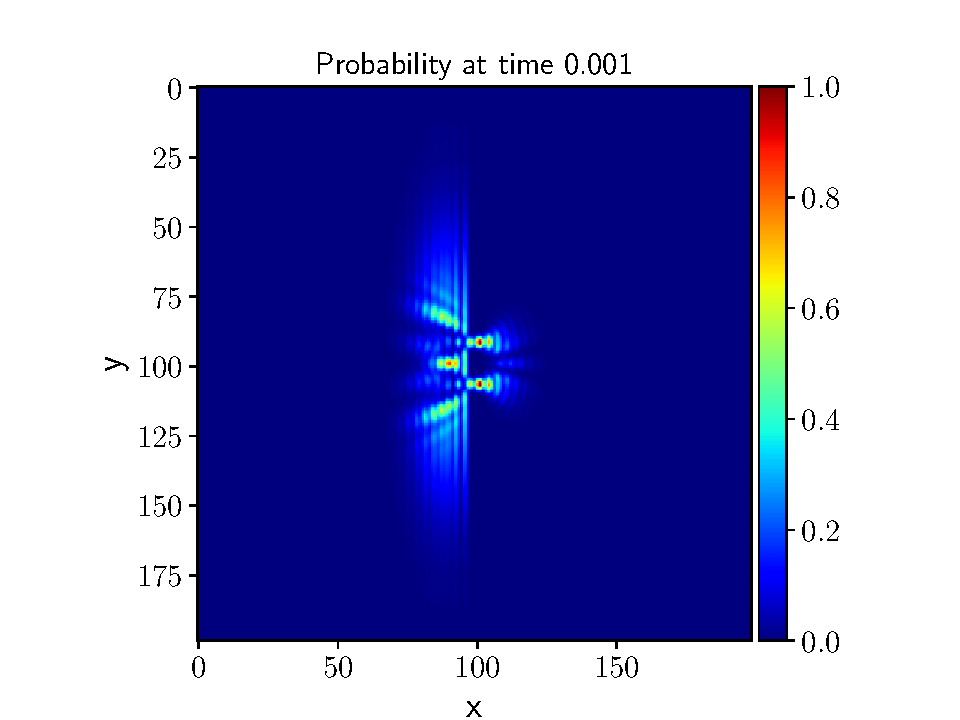
\includegraphics[trim={1cm 0cm 1cm 0cm},clip,width=0.49\textwidth]{figures/prob_plot_0.001.pdf}
		\caption{}
		\label{fig:prob8_P1}
	\end{figure}
	The simulation is run until time $t=2\cross10^{-3}$, which can be seen in figure \ref{fig:prob8_P2}.

	\begin{figure}[H]
		\centering
		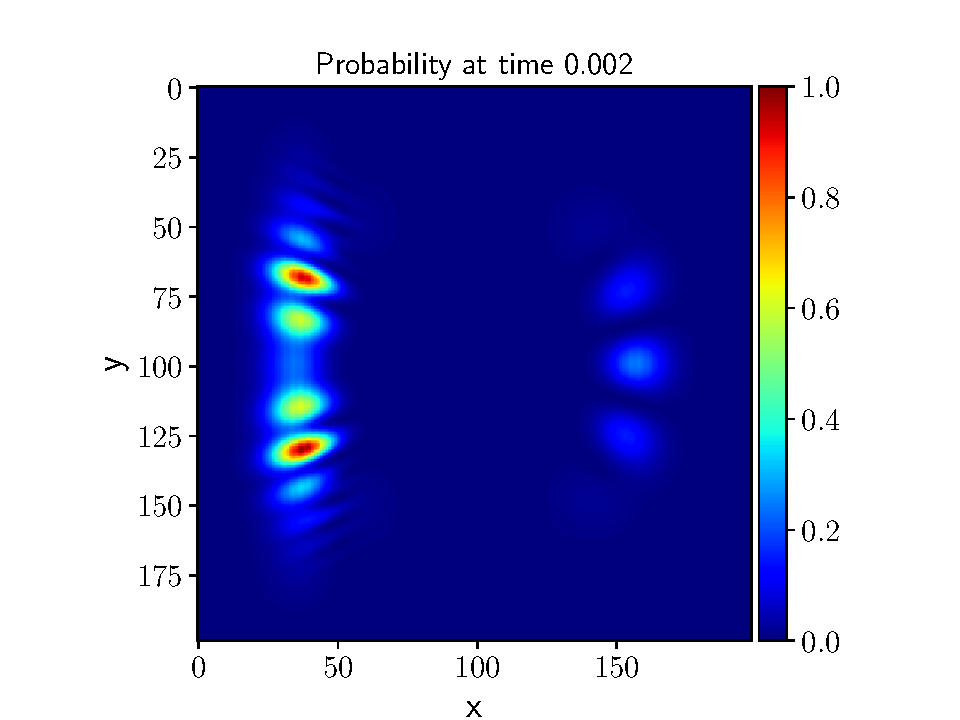
\includegraphics[trim={1cm 0cm 1cm 0cm},clip,width=0.49\textwidth]{figures/prob_plot_0.002.pdf}
		\caption{}
		\label{fig:prob8_P2}
	\end{figure}
	We observe the probability bounces back from the "infinite" potentials of the walls. Next up we will look at how the real and imaginary parts of the Schrödinger equation evolves. The real part of the dimensionless wave function $u$, and how it evolves with time $t \in[0, 2\cross10^{-3}]$ can be seen in figure \ref{fig:prob8_Re0}, \ref{fig:prob8_Re1} and \ref{fig:prob8_Re2}.

	\begin{figure}[H]
		\centering
		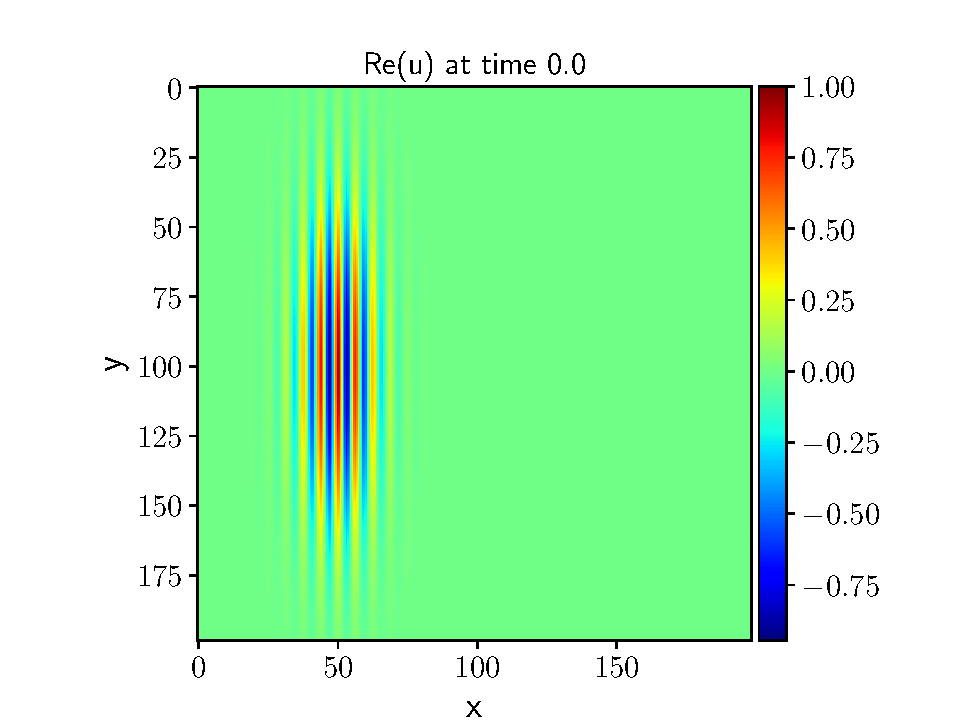
\includegraphics[trim={1cm 0cm 1cm 0cm},clip,width=0.49\textwidth]{figures/real_plot_0.0.pdf}
		\caption{The real part of the wave function $u$ at time $t = 0$.}
		\label{fig:prob8_Re0}
	\end{figure}

	\begin{figure}[h!]
		\centering
		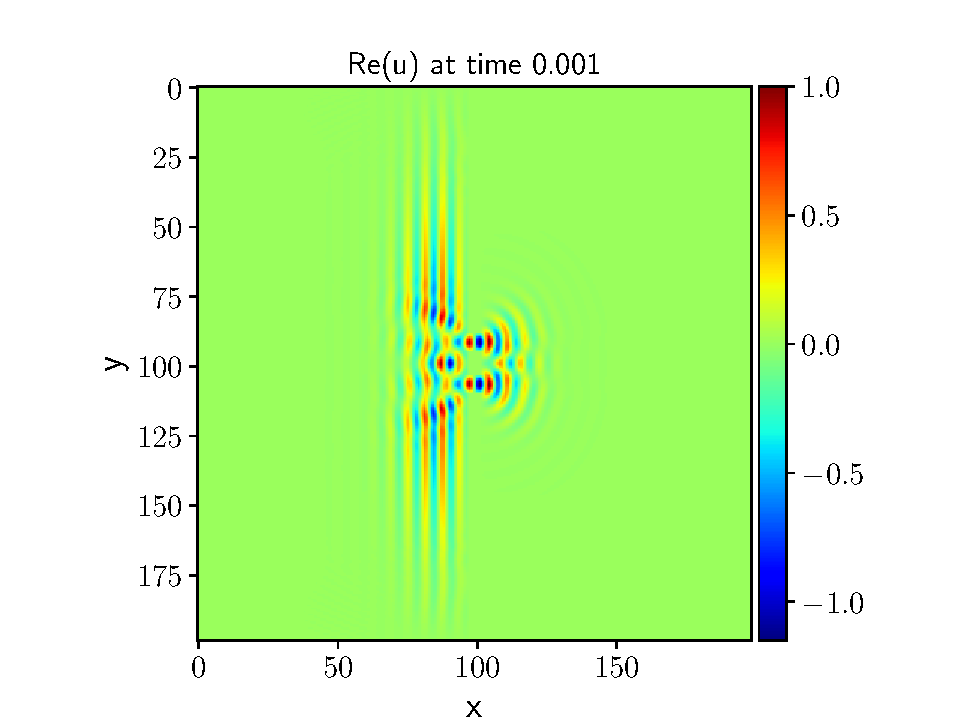
\includegraphics[trim={1cm 0cm 1cm 0cm},clip,width=0.49\textwidth]{figures/real_plot_0.001.pdf}
		\caption{The real part of the wave function $u$ at time $t = 10^{-3}$.}
		\label{fig:prob8_Re1}
	\end{figure}

	\begin{figure}[h!]
		\centering
		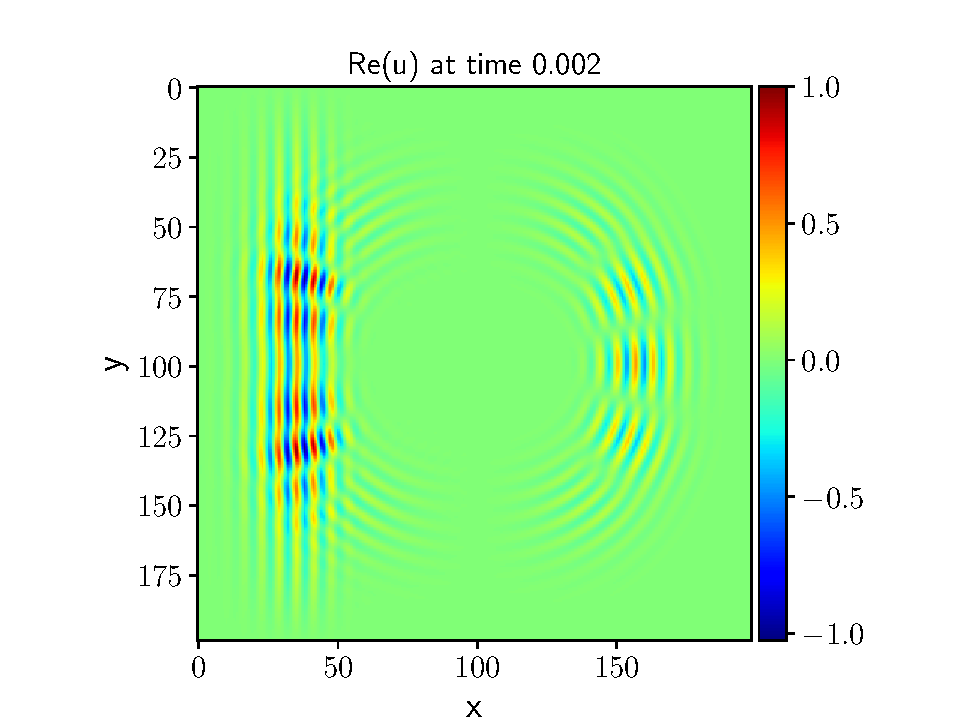
\includegraphics[trim={1cm 0cm 1cm 0cm},clip,width=0.49\textwidth]{figures/real_plot_0.002.pdf}
		\caption{The real part of the wave function $u$ at time $t = 2\cross10^{-3}$.}
		\label{fig:prob8_Re2}
	\end{figure}
	We then look at the imaginary part at the equal times.
	\begin{figure}[h!]
		\centering
		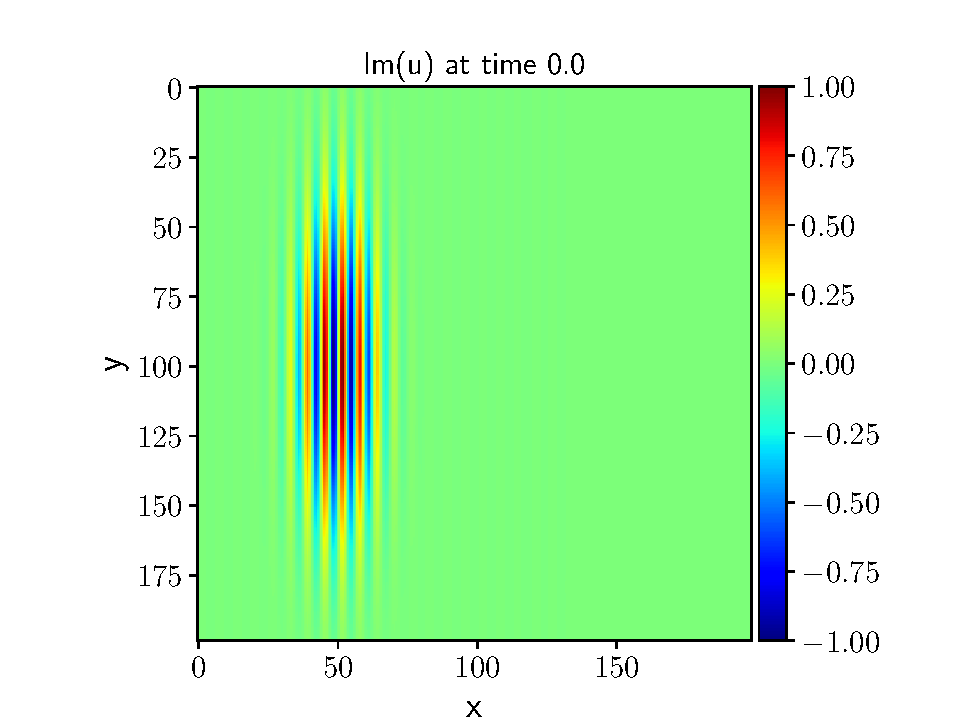
\includegraphics[trim={1cm 0cm 1cm 0cm},clip,width=0.49\textwidth]{figures/im_plot_0.0.pdf}
		\caption{The imaginary part of the wave function $u$ at time $t = 0$}
		\label{fig:prob8_Im0}
	\end{figure}
	
	\begin{figure}[h!]
		\centering
		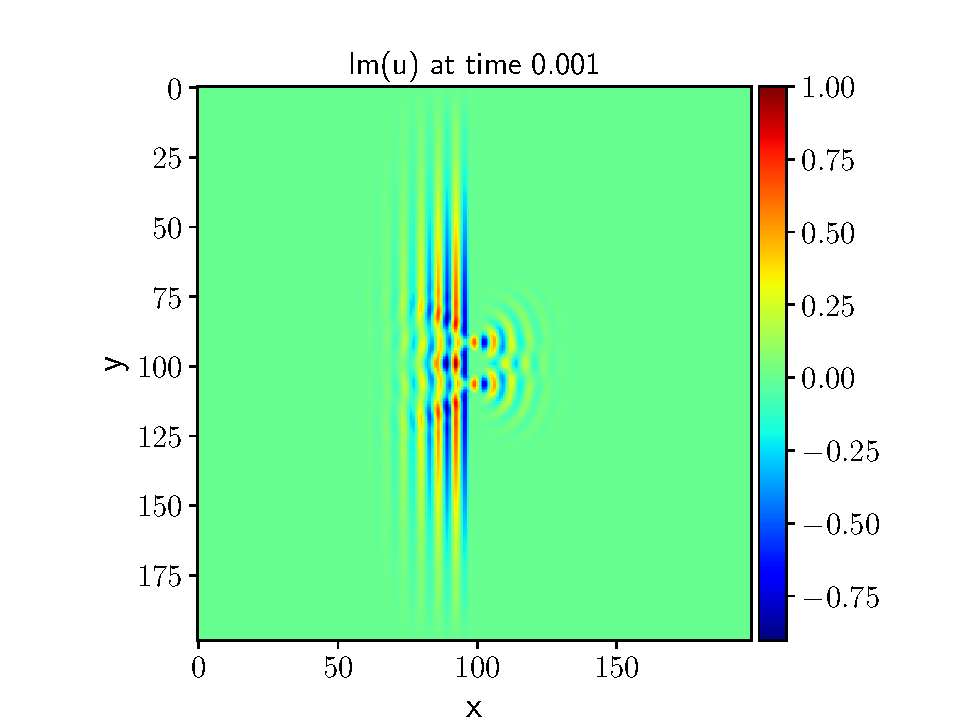
\includegraphics[trim={1cm 0cm 1cm 0cm},clip,width=0.49\textwidth]{figures/im_plot_0.001.pdf}
		\caption{The imaginary part of the wave function $u$ at time $t = 10^{-3}$}
		\label{fig:prob8_Im1}
	\end{figure}
	
	\begin{figure}[h!]
		\centering
		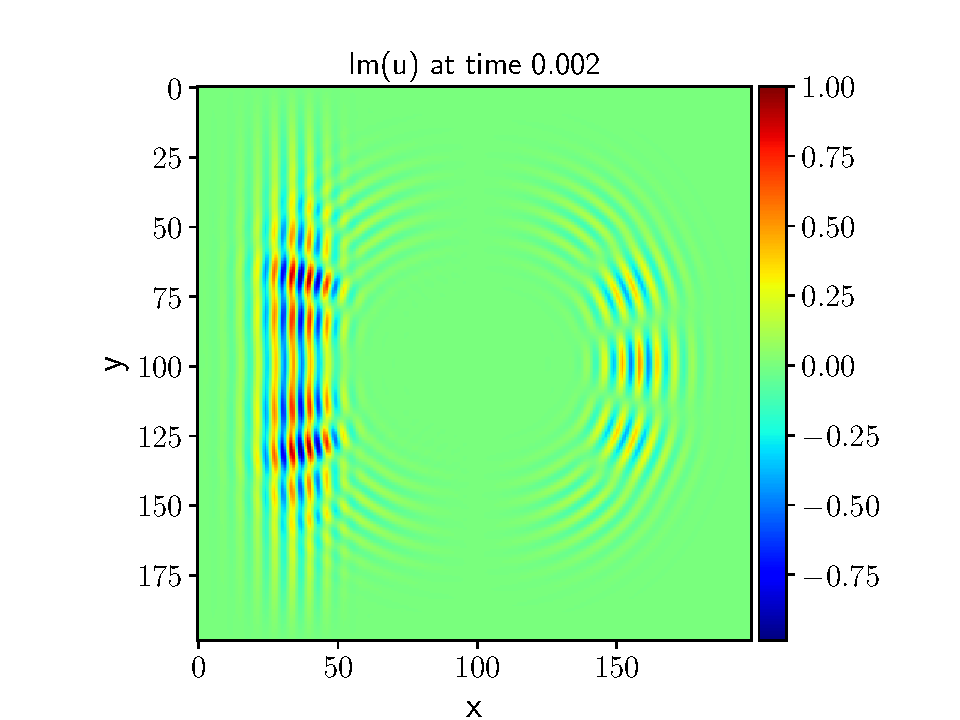
\includegraphics[trim={1cm 0cm 1cm 0cm},clip,width=0.49\textwidth]{figures/im_plot_0.002.pdf}
		\caption{The imaginary part of the wave function $u$ at time $t = 2\cross10^{-3}$}
		\label{fig:prob8_Im2}
	\end{figure}

	\begin{figure}[h!]
		\centering
		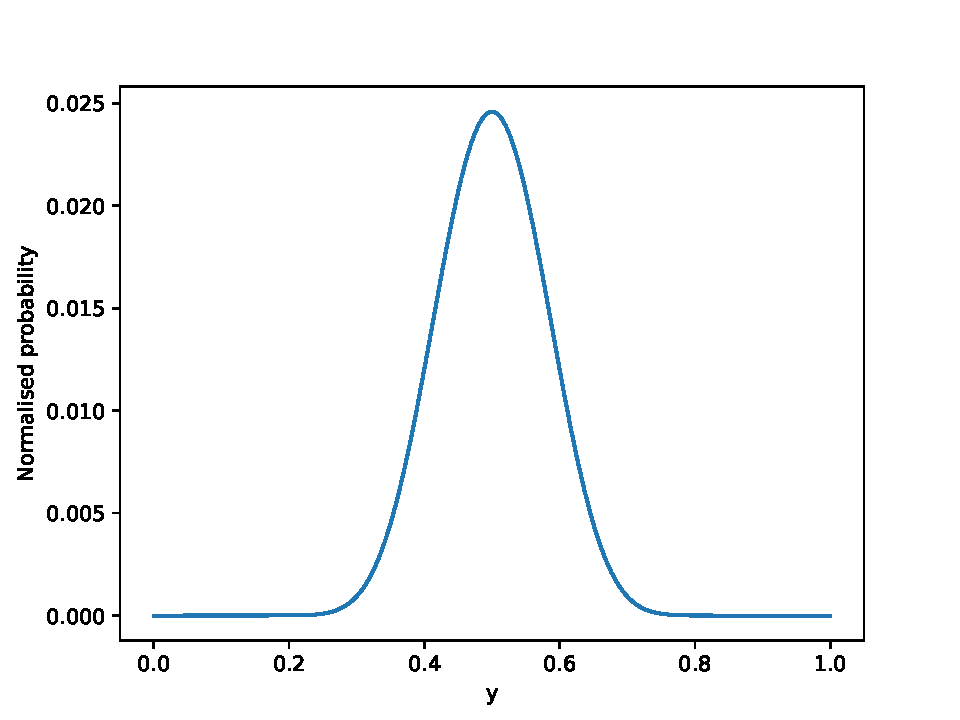
\includegraphics[scale=0.55]{figures/single_slit_detection.pdf}
		\caption{}
		\label{fig:prob9_single}
	\end{figure}
	
	\begin{figure}[h!]
		\centering
		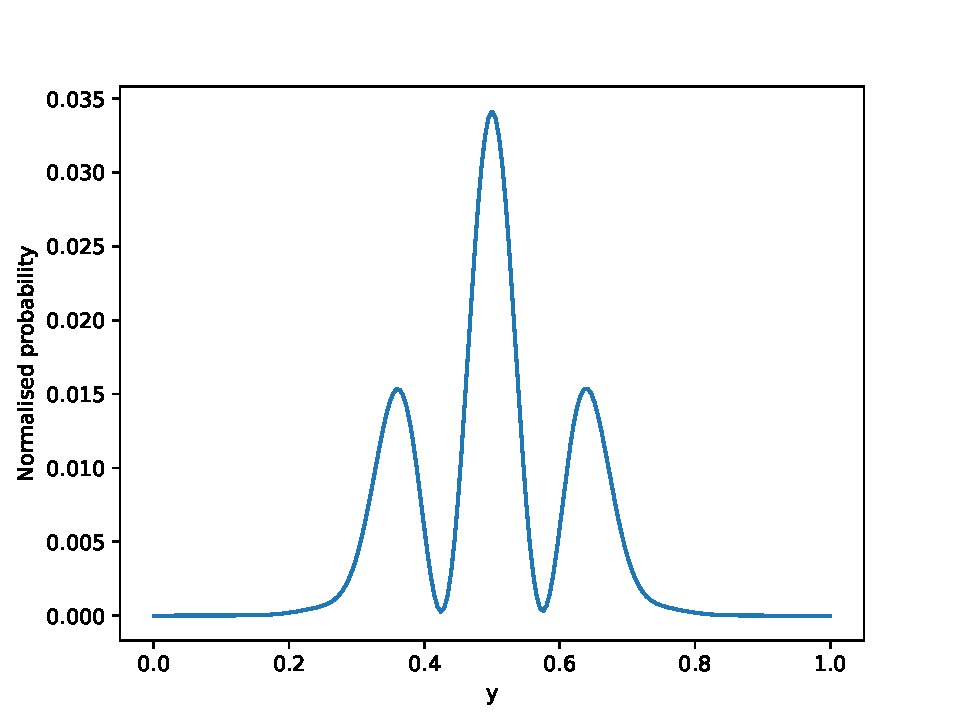
\includegraphics[scale=0.55]{figures/double_slit_detection.pdf}
		\caption{}
		\label{fig:prob9_double}
	\end{figure}
	
	\begin{figure}[H]
		\centering
		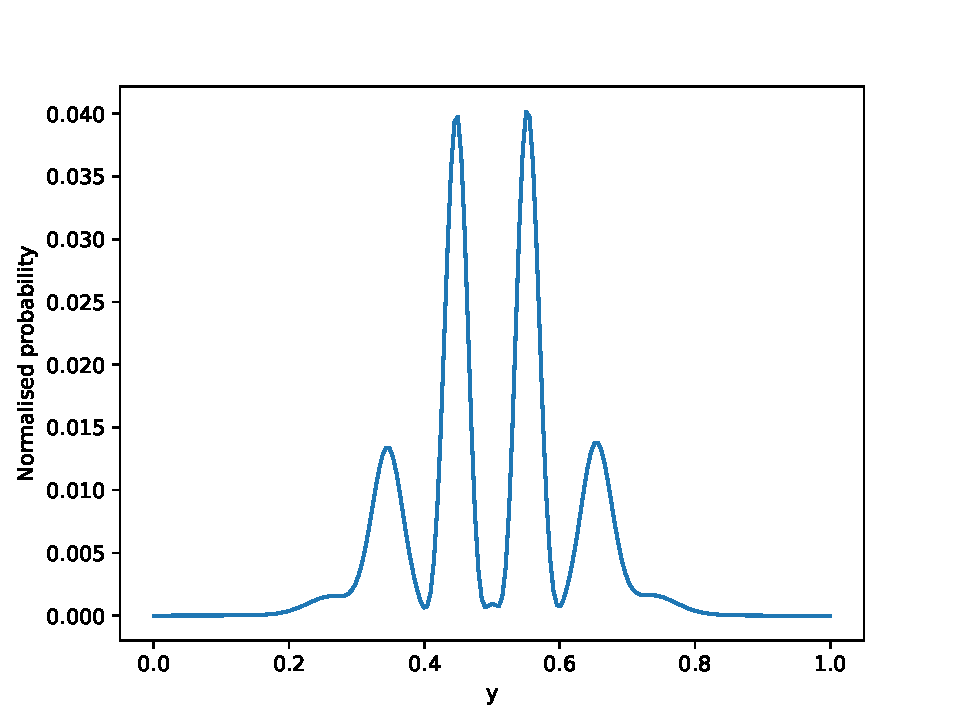
\includegraphics[scale=0.55]{figures/triple_slit_detection.pdf}
		\caption{}
		\label{fig:prob9_triple}
	\end{figure}

	% ===========================================
	\section{Discussion}\label{sec:discussion}
	% ===========================================
	
	\subsection{Total probability deviation} \label{subsec:tot_prob_dev}
	
	One important aspect of numerical analysis is to make sure our numerical
	solution does not diverge. It is a crucial aspect especially when no 
	analytical solutions exist or are known. For example, in case of an 
	Newtonian system of equation, we usually have conservation of energy
	so checking that our energy is conserved is a good indicator that our
	results are significant. In the case of quantum mechanics, since we 
	can only observe probabilities one good convergence check is to make sure
	that our total probability is 1 at all time during our simulation. \\
	
	In Fig.	\ref{fig:prob7_error}, we have plotted the absolute error of 
	the total probability $|P_{\rm tot} - 1|$ for all time step. 
	We see that our total probability is always close to the theoretical 
	value of 1 with an error margin of $10^{-14}$.  \\
	
	We made a function in our python script to make sure that all further 
	simulation also pass our benchmark. 
	
	\subsection{Color-map of the wave-function and probability distribution}\label{subsec:colormap}
	
	Now we have run a simulation with the parameters for the double-slit found in
	Table \ref{tab:1} and we have plotted the Real, Imaginary and the probability
	distribution for times $t \in \{0, 0.001, 0.002 \}$s. All colorbar have been 
	normalized to the maximum value in each plot. \\
	
	At $t=0$ Figures \ref{fig:prob8_Im0}, \ref{fig:prob8_Re0} and \ref{fig:prob_P0}
	shows respectively the imaginary, real part and the distribution probability 
	of our initial Gaussian wave-packet. We also notice that the Real and Imaginary 
	part have opposite value making the complex-norm looking like our probability
	distribution as expected. \\
	
	At $t=0.001$ Figures \ref{fig:prob8_Im1}, \ref{fig:prob8_Re1} and \ref{fig:prob8_P1}
	represent our particle hitting the double-slit configuration. We first see that our 
	particle only moved in the $x$-direction as it makes sense because we only gave a 
	momentum in that direction. When our particle it the slit configuration we can see 
	that it behaves like a wave with some part being reflected with negative and positive 
	value due to the constructive or destructive interference pattern. On the other side
	we can see part of the wave went through the slit but has not interacted with itself 
	yet. \\ 
	
		
	The plot for our final time stamp $t=0.002$ are represented by 
	Figures \ref{fig:prob8_Im2}, \ref{fig:prob8_Re2} and \ref{fig:prob8_P2}
	That time shows the wave function after it has passed the slit configuration. 
	We now observe interference pattern in both reflected and transmitted part. This 
	is expected as a wave will interact with itself. We can see that the particle has
	greater probability of being reflected than moving through, due to the size difference
	between the slit aperture and the wall. We can observe two spots of high probability in 
	the reflected part around ($x\approx0.3$, $y\approx0.60$ and $y\approx0.30$). This is 
	probably due to the constructive interference. 
	
	On the transmitted part we see three main region with one more probable than the other 
	two. The wave spreading creates interference pattern meaning that we observe minima and 
	maxima. \\
	
	The Real and Imaginary part of the wave-function can not be describe physically as it 
	is not possible to observe it. We can only give some sense in our case when we put them
	together by calculating the complex norm giving us the probability distribution. We can 
	see from all Imaginary and Real part that they 'follow' the behavior of our wave as 
	expected. 
	
	
	\subsection{Detection Probability} \label{subsec:detec_prob}
	
	One last interesting thing we look at is the detection probability of our particle. 
	For simulating this we imagine a detector screen at $x=0.8$ and we took the probability
	distribution along that line. We assume that we detect the particle so we normalized 
	our "line-distribution" so that the sum of all probability goes to 1. We used this method
	for our three slit configuration plotted in Figures \ref{fig:prob9_single} \ref{fig:prob9_double}
	and \ref{fig:prob9_triple}. \\
	
	For the single slit we see a Gaussian shape-like profile around the center where the slit
	is. In that case the wave interact with itself but no interference are present.	For the
	double slit we see one maxima at the center and two secondary maxima on the edges. We now
	start to observe some interference pattern due to slit configuration making the wave 
	interfere constructively on the maxima and destructively in between the pics. Finally for
	the triple slit we observe once again interference pattern with four maxima and three 
	minima. However we do not observe the maxima to be around the center in that case. One 
	interesting thing to do would be to use the classical wave equation and solve the 
	slit-configuration and compare with our results. 
	
	
	
	% ===========================================
	\section{Conclusion}\label{sec:conclusion}
	% ===========================================
	
	In this paper we simulated a single non-relativistic particle obeying 
	Schrodinger's equation through three types of slit setup, single, double
	or triple slit. We observed that going through a slit most of the wave-
	function was reflected while a small part passed through. We saw the 
	interference pattern characteristic for a wave. \\
	
	We also represented the detection probability if we would have placed 
	a detector screen behind the wall at $x=0.8$. We found maxima and 
	minima due to constructive or destructive interference. \\
	
	All simulation passed the convergence check by conserving the total 
	probability value with a negligible error of order  $10^{-14}$. \\
	
	
	
	\onecolumngrid
	\section*{References}
	%\bibliographystyle{apalike}
	\bibliography{refs}
	
	
\end{document}
